
\chapter{The Load/Store Unit (LSU)}\label{sec:lsu}

The Load/Store Unit is responsible for deciding when to fire memory operations to the memory system.  There are three queues: the Load Address Queue (LAQ), the Store Address Queue (SAQ), and the Store Data Queue (SDQ).  Load instructions generate a ``uopLD" micro-op.  When issued, ``uopLD" calculates the load address and places its result in the LAQ.  Store instructions (may) generate {\em two} micro-ops,  ``uopSTA" (Store Address Generation) and ``uopSTD" (Store Data Generation).  The STA micro-op calculates the store address and places its result in the SAQ queue.  The STD micro-op moves the store data from the register file to the SDQ.  Each of these micro-ops will issue out of the {\em Issue Window} as soon their operands are ready.  See Section \ref{sec:storeuops} for more details on the store micro-op specifics. 

\subsection{Store Instructions}

Entries in the Store Queue\footnote{When I refer to the {\em Store Queue}, I really mean both the SAQ and SDQ.} are allocated in the {\em Decode} stage (the appropriate bit in the {\tt stq\_entry\_val} vector is set).  A ``valid" bit denotes when an entry in the SAQ or SDQ holds a valid address or data ({\tt saq\_val} and {\tt sdq\_val} respectively).  Once a store instruction is committed, the corresponding entry in the Store Queue is marked as committed.  The store is then free to be fired to the memory system at its convenience.  Stores are fired to the memory in program order.


\subsection{Store Micro-ops}\label{sec:storeuops}

Stores are inserted into the issue window as a single instruction (as opposed to being broken up into separate {\tt addr-gen} and {\tt data-gen} micro-ops). This prevents wasteful usage of the expensive issue window entries and extra contention on the issue port to the LSU.  A store in which both operands are ready can be issued to the LSU as a single micro-op which provides both the address and the data to the LSU.  While this requires store instructions to have access to two register file read ports, this is motivated by a desire to not cut performance in half on store-heavy code.  Sequences involving stores to the stack should operate at IPC=1!

However, it is common for store addresses to be known well in advance of the store data.  Store addresses should be moved to the SAQ as soon as possible to allow later loads to avoid any memory ordering failures. Thus, the issue window will emit uopSTA or uopSTD micro-ops as required, but retain the remaining half of the store until the second operand is ready.

\subsection{Load Instructions}

Entries in the Load Queue (LAQ) are allocated in the {\em Decode} stage ({\tt laq\_entry\_val}).  In {\em Decode}, each load entry is also given a {\em store mask} ({\tt laq\_st\_mask}), which marks which stores in the Store Queue the given load depends on.  When a store is fired to memory and leaves the Store Queue, the appropriate bit in the {\em store mask} is cleared.

Once a load address has been computed and placed in the LAQ, the corresponding {\em valid} bit is set ({\tt laq\_val}). 

Loads are optimistically fired to memory on arrival to the LSU (getting loads fired early is a huge benefit of out--of--order pipelines).  Simultaneously, the load instruction compares its address with all of the store addresses that it depends on.  If there is a match, the memory request is killed.  If the corresponding store data is present, then the store data is {\em forwarded} to the load and the load marks itself as having {\em succeeded}.  If the store data is not present, then the load goes to {\em sleep}.  Loads that have been put to sleep are retried at a later time.\footnote{Higher-performance processors will track {\em why} a load was put to sleep and wake it up once the blocking cause has been alleviated.}


\subsection{Memory Ordering Failures}

The Load/Store Unit has to be careful regarding {\tt store$\rightarrow$load} dependences.  For the best performance, loads need to be fired to memory as soon as possible. 

\begin{quote}

{\texttt
sw x1 $\rightarrow$ 0(x2)

ld x3 $\leftarrow$ 0(x4)
}

\end{quote}


However, if {\tt x2} and {\tt x4} reference the same memory address, then the load in our example {\em depends} on the earlier store.  If the load issues to memory before the store has been issued, the load will read the wrong value from memory, and a {\em memory ordering failure} has occurred.  On an ordering failure, the pipeline must be flushed and the rename map tables reset.  This is an incredibly expensive operation.

To discover ordering failures, when a store commits, it checks the entire LAQ for any address matches.  If there is a match, the store checks to see if the load has {\em executed}, and if it got its data from memory or if the data was forwarded from an older store.  In either case, a memory ordering failure has occurred.  

See Figure \ref{fig:lsu} for more information about the Load/Store Unit.

\


\begin{figure}[ht]
	\centering
	\centerline{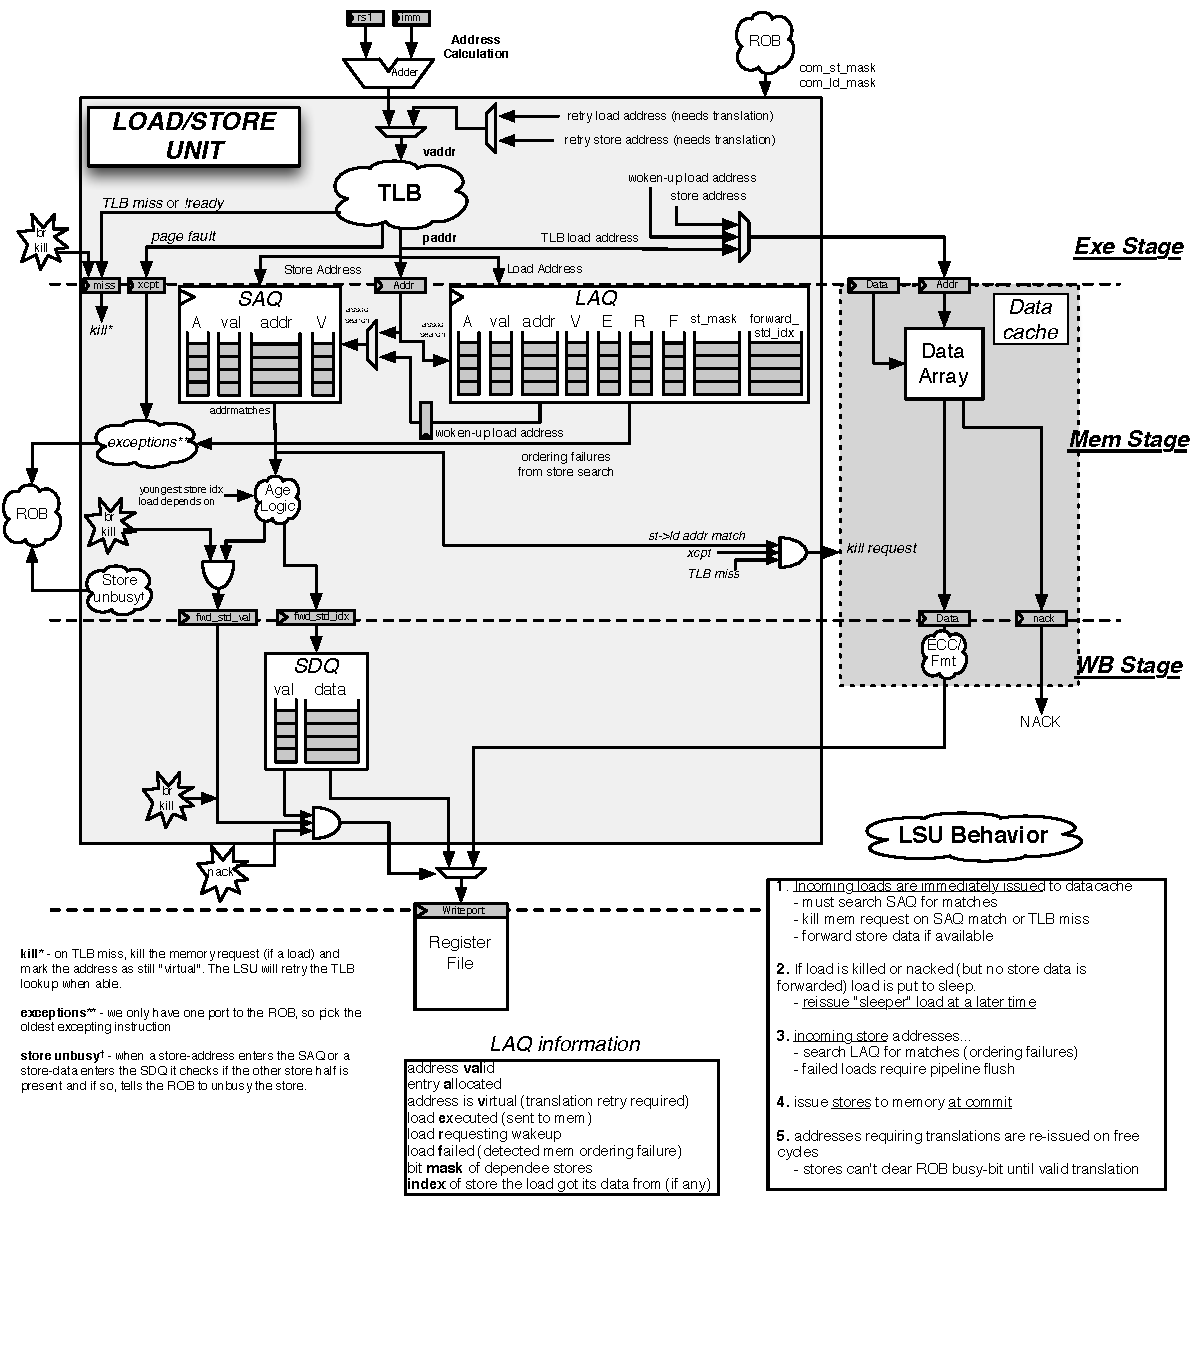
\includegraphics[scale =.9] {figures/lsu}}
	\caption{ \small The Load/Store Unit.}
	\label{fig:lsu}
\end{figure}
